\documentclass[tikz,border=6pt]{standalone}
\usepackage{tikz}
\usetikzlibrary{arrows.meta,positioning}
\definecolor{navy}{HTML}{1E2B55}
\definecolor{blue}{HTML}{1769AA}
\definecolor{gold}{HTML}{B8860B}
\begin{document}
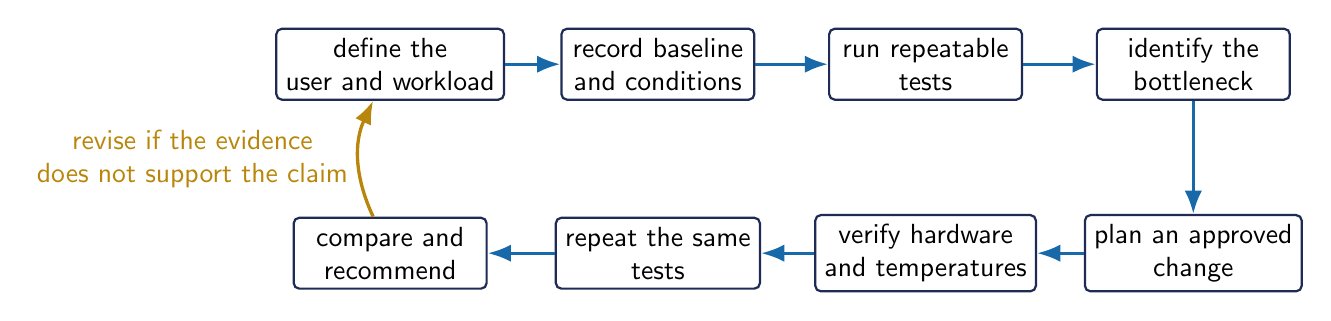
\begin{tikzpicture}[font=\sffamily,>=Latex]
  \tikzset{flowbox/.style={draw=navy,thick,rounded corners=2pt,minimum width=2.45cm,minimum height=0.9cm,align=center,fill=white}}
  \node[flowbox] (purpose) at (0,0) {define the\\user and workload};
  \node[flowbox] (baseline) at (3.4,0) {record baseline\\and conditions};
  \node[flowbox] (test) at (6.8,0) {run repeatable\\tests};
  \node[flowbox] (bottle) at (10.2,0) {identify the\\bottleneck};
  \node[flowbox] (plan) at (10.2,-2.4) {plan an approved\\change};
  \node[flowbox] (verify) at (6.8,-2.4) {verify hardware\\and temperatures};
  \node[flowbox] (retest) at (3.4,-2.4) {repeat the same\\tests};
  \node[flowbox] (explain) at (0,-2.4) {compare and\\recommend};
  \draw[blue,very thick,->] (purpose)--(baseline);
  \draw[blue,very thick,->] (baseline)--(test);
  \draw[blue,very thick,->] (test)--(bottle);
  \draw[blue,very thick,->] (bottle)--(plan);
  \draw[blue,very thick,->] (plan)--(verify);
  \draw[blue,very thick,->] (verify)--(retest);
  \draw[blue,very thick,->] (retest)--(explain);
  \draw[gold,very thick,->] (explain) to[bend left=25] node[left,align=center]{revise if the evidence\\does not support the claim} (purpose);
\end{tikzpicture}
\end{document}
